% GENERATED by scripts/make_figures.py from report/data/report_data.json. Do not edit; regenerate.
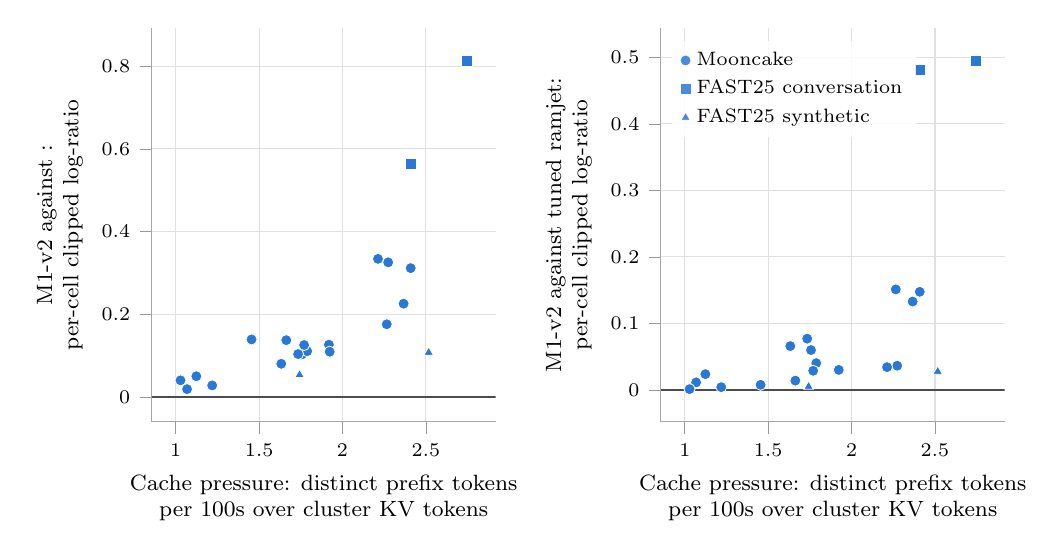
\begin{tikzpicture}
\begin{axis}[
  name=cpleft, width=0.36\linewidth, height=5cm,
  scale only axis,
  tick label style={font=\scriptsize}, label style={font=\footnotesize, align=center},
  scaled ticks=false, tick label style={/pgf/number format/fixed},
  tick align=outside, tick style={black!40}, axis line style={black!35},
  axis x line*=bottom, axis y line*=left,
  grid style={black!12, line width=0.4pt},
  legend style={font=\scriptsize, draw=none, fill=white, fill opacity=0.85, text opacity=1},
  legend cell align=left,
  xmajorgrids, ymajorgrids,
  xlabel={Cache pressure: distinct prefix tokens\\per \SI{100}{s} over cluster KV tokens},
  ylabel={M1-v2 against $\piref$:\\per-cell clipped log-ratio},
  legend style={at={(0.03,0.97)}, anchor=north west},
]
% data: m1v2_vs_default.mooncake
\addplot[only marks, mark=*, mark size=2pt, color={rgb,255:red,42;green,120;blue,214}, mark options={draw=white, line width=0.3pt}] coordinates {(1.662958140449599,0.13708390767366896) (1.0680760685676352,0.018646406968525556) (1.6327814944122352,0.07995279545473953) (1.0286424788258663,0.03989846465962922) (1.4547737975445036,0.13884600978444242) (1.7568570238818544,0.10262799355010817) (1.788177257758446,0.11033075922171198) (1.2187942040011592,0.027547199298678087) (1.7698128964987982,0.12529955098768272) (1.1236368797472236,0.049837815536242724) (2.27379730163919,0.32532798548627595) (2.265171425760735,0.1755062294570351) (2.2126246816380544,0.3336922585193361) (2.3662919853556668,0.22531435015965282) (2.408794738186328,0.31130885052082835) (1.9184876936042667,0.12626656708396325) (1.7338384858513693,0.10350587082541106) (1.9232627723458995,0.1091367587244521)};
% data: m1v2_vs_default.fast25_conversation
\addplot[only marks, mark=square*, mark size=2pt, color={rgb,255:red,42;green,120;blue,214}, mark options={draw=white, line width=0.3pt}] coordinates {(2.410181047818837,0.5636409873887084) (2.7458641097979104,0.8122643249485385)};
% data: m1v2_vs_default.fast25_synthetic
\addplot[only marks, mark=triangle*, mark size=2pt, color={rgb,255:red,42;green,120;blue,214}, mark options={draw=white, line width=0.3pt}] coordinates {(2.5165505977424956,0.10728519098403601) (1.7425118339794181,0.05327629154274147)};
\draw[black!70, line width=0.6pt] ({rel axis cs:0,0} |- {axis cs:0,0.0}) -- ({rel axis cs:1,0} |- {axis cs:0,0.0});
\end{axis}
\begin{axis}[
  at={(cpleft.south east)}, anchor=south west, xshift=2.1cm, width=0.36\linewidth, height=5cm,
  scale only axis,
  tick label style={font=\scriptsize}, label style={font=\footnotesize, align=center},
  scaled ticks=false, tick label style={/pgf/number format/fixed},
  tick align=outside, tick style={black!40}, axis line style={black!35},
  axis x line*=bottom, axis y line*=left,
  grid style={black!12, line width=0.4pt},
  legend style={font=\scriptsize, draw=none, fill=white, fill opacity=0.85, text opacity=1},
  legend cell align=left,
  xmajorgrids, ymajorgrids,
  xlabel={Cache pressure: distinct prefix tokens\\per \SI{100}{s} over cluster KV tokens},
  ylabel={M1-v2 against tuned \policy{ramjet}:\\per-cell clipped log-ratio},
  legend style={at={(0.03,0.97)}, anchor=north west},
]
% data: m1v2_vs_ramjet.mooncake
\addplot[only marks, mark=*, mark size=2pt, color={rgb,255:red,42;green,120;blue,214}, mark options={draw=white, line width=0.3pt}] coordinates {(1.662958140449599,0.014026222433940293) (1.0680760685676352,0.01128173558192431) (1.6327814944122352,0.06588797115852886) (1.0286424788258663,0.001203984777751311) (1.4547737975445036,0.007637622884751107) (1.7568570238818544,0.05990092738100362) (1.788177257758446,0.0402384326279203) (1.2187942040011592,0.004156519149548524) (1.7698128964987982,0.028756639487820635) (1.1236368797472236,0.02371316423989103) (2.27379730163919,0.036397844915040854) (2.265171425760735,0.15108987884710914) (2.2126246816380544,0.03425018661221003) (2.3662919853556668,0.13285757078023258) (2.408794738186328,0.147493683985517) (1.9184876936042667,0.030136199397582886) (1.7338384858513693,0.07705811989834781) (1.9232627723458995,0.030121008600834387)};
\addlegendentry{Mooncake}
% data: m1v2_vs_ramjet.fast25_conversation
\addplot[only marks, mark=square*, mark size=2pt, color={rgb,255:red,42;green,120;blue,214}, mark options={draw=white, line width=0.3pt}] coordinates {(2.410181047818837,0.481465018099776) (2.7458641097979104,0.4943816448038311)};
\addlegendentry{FAST25 conversation}
% data: m1v2_vs_ramjet.fast25_synthetic
\addplot[only marks, mark=triangle*, mark size=2pt, color={rgb,255:red,42;green,120;blue,214}, mark options={draw=white, line width=0.3pt}] coordinates {(2.5165505977424956,0.027708508068614426) (1.7425118339794181,0.005070687323773607)};
\addlegendentry{FAST25 synthetic}
\draw[black!70, line width=0.6pt] ({rel axis cs:0,0} |- {axis cs:0,0.0}) -- ({rel axis cs:1,0} |- {axis cs:0,0.0});
\end{axis}
\end{tikzpicture}
